\documentclass[aspectratio=169,10pt]{beamer}
\usepackage{pgf}
\usepackage{colortbl,tabularx,amsfonts,mathrsfs,calligra}
\usepackage{ragged2e}
\usepackage{setspace}
\usepackage{tikz}
\usepackage{filecontents}
\usepackage{xcolor}
\usepackage{caption}
\usepackage{subcaption}
\usepackage{contour}
\usepackage{fancybox}
\usepackage{wrapfig}
\usepackage{multirow}
\usepackage{multicol}
\usepackage{tikz, pgfplots, tkz-euclide,calc}
    \usetikzlibrary{patterns,snakes,shapes.arrows}
\usepackage{listings}
    
\definecolor{langit}{HTML}{FAEDC8}
\definecolor{permukaan}{HTML}{E3BF90}
\definecolor{tanah}{HTML}{F4965B}
\definecolor{box}{HTML}{5C2921}
\definecolor{header}{HTML}{0F5165}
\definecolor{bgcode}{HTML}{B2AAA0}
\definecolor{omitscyan}{HTML}{15EBD6}
\definecolor{oren}{HTML}{F67D49}

\lstdefinestyle{myStyle}{
        belowcaptionskip    =0.5\baselineskip,
        breaklines          =true,
        frame               =single,
        basicstyle          =\footnotesize\ttfamily,
        language            =[LaTeX]{TeX},
        keywordstyle        =\bfseries\color{green!40!black},
        commentstyle        =\itshape\color{purple!40!black},
        identifierstyle     =\color{blue},
        backgroundcolor     ={\color{bgcode}},
        numbers             = left, % {none, left, right}
        numberstyle         = \scriptsize\color{black},
        numbersep           = -8pt,
        frame               =shadowbox, 
        rulesepcolor        =\color{box},
    }
\lstset{style=mystyle}


\bibliographystyle{apalike}
\usetheme{Madrid}
\usecolortheme[named=header]{structure}

\usefonttheme{professionalfonts}
\setbeamertemplate{theorems}[numbered]
\setbeamertemplate{bibliography item}{\insertbiblabel}
\setbeamercovered{transparent}

\setbeamercolor{boxcoklat}{fg=langit,bg=header}
\setbeamercolor{boxpurple}{fg=white,bg=purple}
\setbeamercolor{boxpink}{fg=black,bg=pink}
\setbeamercolor{boxviolet}{fg=white,bg=violet}
\setbeamercolor{boxabu}{fg=black!30!blue!100,bg=gray!40}
\usebackgroundtemplate{\includegraphics[width=\paperwidth]{bgPPT.jpg}}

\renewcommand\thesubfigure{\arabic{subfigure}}
\newtheorem{definisi}{Definisi}
\newtheorem{funfact}{Fun Fact}
\newtheorem{latihan}{Latihan \LaTeX}
\AtBeginEnvironment{funfact}{%
  \setbeamercolor{block title}{use=example text,fg=white,bg=example text.fg!75!black}
  \setbeamercolor{block body}{parent=normal text,use=block title example,bg=block title example.bg!10!bg}
}
\AtBeginEnvironment{latihan}{%
  \setbeamercolor{block title}{use=example text,fg=white,bg=omitscyan!50!black}
  \setbeamercolor{block body}{parent=normal text,use=block title example,bg=omitscyan!10!white}
}



 \pgfdeclareimage[height=.85cm]{logo}{logoOMITS}
 \logo{\pgfuseimage{logo}}

\date{}
\title{Olimpiade Matematika ITS 17th}
\author{Upgrading Latex}
\institute{QM}



\begin{document}

{\usebackgroundtemplate{\includegraphics[width=\paperwidth,height=\paperheight]{titleppt.png}}
    \begin{frame}[plain]
    
    \transboxout

    \begin{beamercolorbox}[wd=\textwidth,rounded=true,shadow=true]{boxcoklat}
        \centering
        \resizebox{.5\textwidth}{1em}{%
        \textsf{\textbf{UPGRADING \LaTeX}}}
    \end{beamercolorbox}

    \vspace*{3ex}

    \centerline{\includegraphics[scale=.035]{logoOMITS}}

    \vspace*{1ex}

    \begin{center}
        \contourlength{1pt}% thickness
        \contournumber{20}% copies used
        \tt
        \contour{black}{\color{langit}QUESTION MAKER}\\
        \contour{black}{\color{langit}OMITS 17th}\\
        \contour{black}{\color{langit}Departemen Matematika ITS}\\
    \end{center}
\end{frame}}

\AtBeginSection[]
{
	\begin{frame}
		\frametitle{Dartar Isi}
		\tableofcontents[hidesubsections,currentsection]
	\end{frame}
}

\section{Pendahuluan}
\begin{frame}
	\transwipe[direction=0]
	\frametitle{Pendahuluan}
	\begin{itemize}
	\item Sering kali saat perkuliahan kita melihat \textbf{PPT/buku} dosen saat 
    beliau menjelaskan suatu materi. Kemudian saat \textbf{ETS}, \textbf{EAS}, atau bahkan 
    \textbf{kuis} kita mendapatkan sebuah \textbf{lembar soal}. Namun pernakah terpikir di 
    pikiran kita "\textbf{Software} apa yang digunakan untuk membuat hal itu?"
    \begin{figure}[h!]
        \centering
        \begin{subfigure}[b]{0.3\linewidth}
          \includegraphics[width=\linewidth]{PPT_pak_fahim.png}
          \caption{PPT dosen}
          \label{fig:PPT}
        \end{subfigure}
        \begin{subfigure}[b]{0.15\linewidth}
          \includegraphics[width=\linewidth]{EAS METMAT 2023.pdf}
          \caption{Soal EAS}
          \label{fig:EAS}
        \end{subfigure}
        \begin{subfigure}[b]{0.17\linewidth}
            \includegraphics[width=\linewidth]{FondasiAljabar.jpg}
            \caption{Buku Aljabar}
            \label{fig:buku}
          \end{subfigure}
    \end{figure}
	\item Saat membuat soal pun perlu adanya suatu struktur baik itu kalimat 
    maupun penyusunannya. Sehingga mempelajari \textbf{\LaTeX} sangat diperlukan
    untuk kedepannya.
	\end{itemize}
\end{frame}

\begin{frame}
    \frametitle{Pendahuluan}
    Motivasi dalam mempelajari \textbf{\LaTeX} adalah untuk menguatkan konsep 
    dan kemampuan dalam \textbf{penulisan dokumen} berlandaskan \textbf{matematika/sains}. 
    Percayalah bahwa dengan belajar \textbf{\LaTeX} akan membantu kita saat 
    menyusun \textbf{Tugas Akhir} nantinya.
\end{frame}

\section{Apa itu \LaTeX}
\begin{frame}
    \frametitle{Apa itu \LaTeX}
    \begin{definisi}
        \textbf{\LaTeX} adalah sistem penyusunan huruf berkualitas tinggi, hal itu mencakup 
        fitur-fitur yang dirancang untuk produksi dokumentasi teknis dan ilmiah. 
        \textbf{\LaTeX} sangat sering digunakan berbagai kalangan mulai dari \textit{Sciencetist}
        hingga \textit{Engineering}. (SC: latex-project.org)
    \end{definisi}
    \begin{figure}[h!]
        \includegraphics[width=0.3\linewidth]{LatexLogo.png}
        \caption{Logo Latex}
    \end{figure}
\end{frame}

\begin{frame}
    \frametitle{Apa itu \LaTeX}
    \begin{figure}
        \begin{subfigure}[t!]{0.3\linewidth}
            \captionsetup{labelformat=empty}
            \caption{\huge{Source}}
            \includegraphics[width=\linewidth]{sourceLatex.png}
        \end{subfigure}
        \begin{subfigure}[t!]{0.3\linewidth}
            \includegraphics[width=\linewidth]{compile.png}
        \end{subfigure}
        \begin{subfigure}[t!]{0.3\linewidth}
            \captionsetup{labelformat=empty}
            \caption{\huge{Result}}
            \includegraphics[width=\linewidth]{resultLatex.png}
        \end{subfigure}
    \end{figure}
\end{frame}

\begin{frame}
    \frametitle{Apa itu \LaTeX}
    \begin{tabularx}{\textwidth}{X X X}
        \textbf{INPUT} & \textbf{PROCESS} & \textbf{OUTPUT} \\
          \begin{itemize}
            \item .tex
            \item .cls
            \item .sty
            \item .pdf, .jpg, .png, etc
          \end{itemize}&
          \begin{itemize}
            \item latex
            \item pdflatex
            \item luatex
            \item xetex
          \end{itemize}&
          \begin{itemize}
            \item .pdf
            \item .log
            \item .aux
            \item .dtx
          \end{itemize}
          \end{tabularx}
\end{frame}
    
\begin{frame}
    \frametitle{Apa itu \LaTeX}
    \begin{funfact}
        Karakter 'T','E',dan 'X' pada namanya berasal dari huruf kapital Yunani 
        kuno: tau($\tau$), epsilon($\epsilon$), chi($\chi$). karena alasan ini, 
        pencipta TeX mempromosikan pengucapannya sebagai \color{blue}tech\color{black}.
        Sehingga \LaTeX$\,$ biasanya dilafalkan dengan \color{blue}{lah-tech}\color{black}.
    \end{funfact}
\end{frame}

\section{\LaTeX$\,$vs MS Word} 
\begin{frame}
    \frametitle{\LaTeX$\,$vs MS Word}
    \begin{center}
        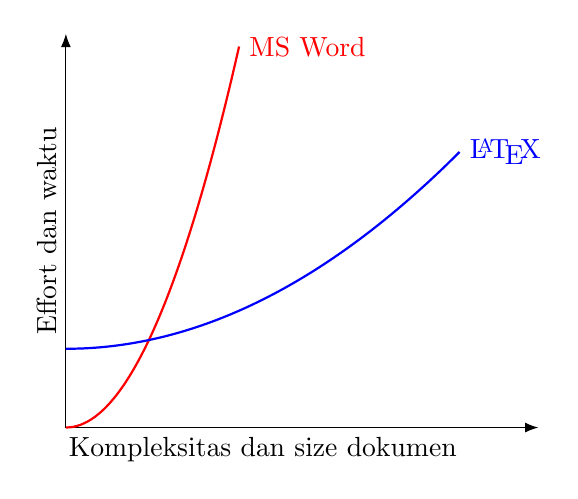
\begin{tikzpicture}
            \draw[-Latex] (0,0) -- (2.5,0) node[below] {Kompleksitas dan size dokumen} --(6,0);
            \draw[-Latex] (0,0) -- (0,2.5) node[left] {\rotatebox{90}{Effort dan waktu}}-- (0,5);
            \draw[thick,red,domain=0:2.2,smooth] plot (\x,{(\x)^2}) node [right] {MS Word};
            \draw[thick,blue,domain=0:5,smooth] plot (\x,{1/10*(\x)^2+1}) node [right] {\LaTeX};
        \end{tikzpicture}
    \end{center}
\end{frame}

\begin{frame}
    \frametitle{\LaTeX$\,$vs MS Word}
    \begin{tabularx}{\textwidth}{X||X|X}
    \textbf{Criterion}&\textbf{MS Word} & \textbf{\LaTeX} \\
      \hline
      Document editing&One editor&Any text editor\\
      Changing format&Entire document& Only class and command\\
      Huge content&Often crash& Stable\\
      \end{tabularx}
\end{frame}

\begin{frame}
    \frametitle{\LaTeX$\,$vs MS Word}
    \begin{figure}
        \begin{subfigure}[t!]{0.6\linewidth}
            \captionsetup{labelformat=empty}
            \caption{MS Word}
            \includegraphics[width=\linewidth]{WordEQ.png}
        \end{subfigure}
        \begin{subfigure}[b!]{0.6\linewidth}
            \captionsetup{labelformat=empty}
            \caption{\LaTeX}
            \includegraphics[width=\linewidth]{LatexEQ.png}
        \end{subfigure}
    \end{figure}
    *Resolusi Simbol Matematika \LaTeX$\,$lebih baik daripada MS word.
\end{frame}

\section{Instalasi \LaTeX} 
\begin{frame}
    \frametitle{Instalasi \LaTeX}
    \begin{tabular}{llll}
        \multicolumn{2}{l}{\textbf{\LaTeX\ OFFLINE}}&\multicolumn{2}{l}{\textbf{\LaTeX\ ONLINE}}\\
        \multirow{3}{*}{\includegraphics[width=0.07\linewidth]{MikTex.png}}&&\multirow{3}{*}{\includegraphics[width=0.07\linewidth]{Overleaf.png}}&\\
        &MikTex (Wajib)&&Overleaf\\
        &&&\\
        \multirow{3}{*}{\includegraphics[width=0.07\linewidth]{texstudio.png}}&&&\\
        &TeXstudio (Text editor)&&\\
        &&&\\
        \multirow{3}{*}{\includegraphics[width=0.07\linewidth]{vscode.png}}&&&\\
        &Visual Studio Code (Text editor)&&\\
        &&&\\
    \end{tabular}
\end{frame}
    
\begin{frame}
    \frametitle{Instalasi \LaTeX (Overleaf)}
    \begin{enumerate}
        \item Akses \color{blue}overleaf.com
        \item \color{black} Sign in menggunakan akun google.
        \item Klik "New Project"
        \item Ketik nama file project
    \end{enumerate}
\end{frame}

\section{Tutorial}
\begin{frame}[fragile]
    \frametitle{Tutorial (1)}
    \begin{lstlisting}[title={Hello World}]
    \documentclass{article}
        
    \begin{document}
        Hello World
    \end{document}
    \end{lstlisting}
    \begin{latihan}
         Ketik contoh diatas dan compile file tex-nya.
    \end{latihan}
\end{frame} 

\begin{frame}[fragile]
    \begin{lstlisting}[title={Struktur},firstnumber=1]
    \documentclass{article} %document class
    \usepackage{amsmath}
    %Command
    ...

    \begin{document}
        Lorem ipsum dolor sit amet...
        %Environment
            ...
            
    \end{document}
    \end{lstlisting}
\end{frame} 
    
\begin{frame}
    \setbeamercolor{block title}{bg=oren, fg=white}
    \setbeamercolor{block body}{bg=oren!10}
    \begin{block}{Document Class}
        Struktur dokumen yang akan dibuat tergantung jenis atau tipe kelas dokumen. Daftar 
        document class \LaTeX:
        \begin{multicols}{3}
            \begin{itemize}
                \item \texttt{article}              
                \item \texttt{report}             
                \item \texttt{book}           
                \item \texttt{beamer}             
                \item \texttt{standalone}
                \item \texttt{letter}         
            \end{itemize}
        \end{multicols}
    \end{block}

    \begin{block}{Command}
        Tidak adanya UI membuat kita perlu mendefinisikan beberapa perintah secara manual. 
        Sehingga menginput sebuah command akan sangat membantu dalam penulisan. Contoh command:
        \begin{multicols}{3}
            \begin{itemize}
                \item \texttt{\string\usepackage\{\}}
                \item \texttt{\string\newcommand<>\{\}[][]\{\}}
                \item \texttt{\string\definecolor[]\{\}}
            \end{itemize}
        \end{multicols}
    \end{block}
\end{frame}

\begin{frame}
    \setbeamercolor{block title}{bg=oren, fg=white}
    \setbeamercolor{block body}{bg=oren!10}
    \begin{block}{Environment}
        Hal yang akan ditampilkan pada dokumen. kita dapat menampilkan tulisan dan gambar pada
        bagian ini. Biasanya diawali \texttt{\string\begin\{...\}} dan diakhiri \texttt{\string\end\{...\}} 
        dengan  Contoh:
        \begin{multicols}{3}
            \begin{itemize}
                \item \texttt{document}                
                \item \texttt{enumerate}
                \item \texttt{align}         
            \end{itemize}
        \end{multicols}
    \end{block}
\end{frame}

\begin{frame}[fragile]
    \frametitle{Tutorial (2)}
    \begin{lstlisting}[title={List item},firstnumber=21]
    \begin{document}

        \begin{enumerate}
            \item Pertanyaan 1
            \item Pertanyaan 2
            \item Pertanyaan 3
        \end{enumerate}
            
    \end{document}
    \end{lstlisting}
\end{frame}

\begin{frame}
    \begin{latihan}
        Ketik contoh soal berikut pada latex anda!
        \begin{figure}[c!]
            \fbox{\includegraphics[width=0.5\textwidth]{contohEnumerate.pdf}}
        \end{figure}
    \end{latihan}
\end{frame}

\begin{frame}
    \setbeamercolor{block title}{bg=oren, fg=white}
    \setbeamercolor{block body}{bg=oren!10}
    \begin{block}{Math's Symbols}
        \texttt{amsmath} adalah salah satu package yang digunakan dalam penulisan matematika
        pada umumnya.
        \begin{center}
            \begin{tabular}{|c|}
                \hline
                \texttt{\string\alpha} $\quad$ \texttt{\string\theta} $\quad$ \texttt{\string\gamma} $\quad$ 
                \texttt{\string\Gamma} $\quad$ \texttt{\string\int} $\quad$ \texttt{\string\sum} 
                $\quad$ \texttt{\string\times} $\quad$ \texttt{\string\cup} $\quad$ \texttt{\string\cap}\\ 

                \texttt{\string\subset} $\quad$ \texttt{\string\subseteq} $\quad$ \texttt{\string\sqrt\{\}} $\quad$ \texttt{\string\frac\{\}\{\}}
                $\quad$ \texttt{\string\pi} $\quad$ \texttt{\string\neq}\\
                \hline
                \hline
                $\alpha \quad \theta \quad \gamma \quad \Gamma \quad \int \quad \sum \quad \times \quad \cup 
                \quad \cap \quad \subset \quad \subseteq \quad \sqrt{...} \quad \theta \quad \frac{.....}{.....} \quad \pi \quad \neq$\\
                \hline
            \end{tabular}
        \end{center}
    \end{block}

    \begin{block}{Math Mode}
        Dalam menulis ekspresi matematika diperlukan sebuah "wadah" untuk menampilkannya agar 
        terlihat lebih estetik. Hal ini dibagi menjadi \color{red}inline \color{black}dan 
        \color{red} display\color{black}.
        \begin{center}
            \begin{tabular}{|c|c|}
                \hline
                \color{red}inline & \color{red}display\\
                \hline
                \texttt{\string\(}\texttt{...}\texttt{\string\)} & \texttt{\string\[}\texttt{...}\texttt{\string\]}\\
                \texttt{\$...\$} & \texttt{\$\$...\$\$}\\
                \hline
            \end{tabular}
        \end{center}
    \end{block}
\end{frame}

\begin{frame}[fragile]
    \frametitle{Tutorial (3)}
    \begin{lstlisting}[title={Math Display},firstnumber=37]
        Carilah $x$ dari $2x-1=0$.\\~\\

        Carilah himpunan penyelesaian
        \[|x-2|\leq 10\]
    \end{lstlisting}
    \begin{figure}[c!]
        \fbox{\includegraphics[width=0.4\textwidth]{contohDisplay.pdf}}
        \captionsetup{labelformat=empty}
        \caption{Output}
    \end{figure}
\end{frame}

\begin{frame}
    \begin{latihan}
        Ketik contoh soal berikut pada latex anda!
        \begin{figure}[c!]
            \fbox{\includegraphics[width=0.5\textwidth]{LatihanDisplay.pdf}}
        \end{figure}
    \end{latihan}
\end{frame}

\begin{frame}[fragile]
    \frametitle{Tutorial (4)}
    \begin{lstlisting}[title={Import n Draw Figure},firstnumber=54]

    \includegraphics[width=...]{...} %type the name of file

    \begin{figure}[]
        \includegraphics[...]{...}
        ...
        \includegraphics[...]{...}
        ...
        ...
        %collection of several images
    \end{figure}

    \begin{tikzpicture}[]
        %syntax for drawing a geometric illustration 
        ...
        ...  
    \end{tikzpicture}

    \end{lstlisting}
\end{frame}

\begin{frame}
    \setbeamercolor{block title}{bg=oren, fg=white}
    \setbeamercolor{block body}{bg=oren!10}
    \begin{block}{Includegraphics}
        Sebuah gambar dapat ditampilkan dalam dokumen dengan cara mengetikkan nama file yang akan
        ditampilkan tersebut. Contoh: \texttt{\string\includegraphics\{LogoOMITS.png\}} 
    \end{block}
    \begin{block}{Tikz}
        Salah satu tools yang cukup sering dipakai dalam membuat ilustrasi geometri. Tidak 
        selamanya saat meng-include sebuah gambar, resolusi saat diprint akan sama saat masih
        menjadi dokumen. Oleh sebab itu, disini cukup \color{red}wajib \color{black}untuk membuat
        sebuah ilustrasi dengan tools yang sudah ada di \LaTeX.
    \end{block}
\end{frame}

\begin{frame}[fragile]
    \begin{lstlisting}[title={Triangle},firstnumber=102]
        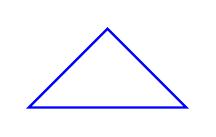
\begin{tikzpicture}[]
            \draw[thick,blue] (0,0)--(1,1)--(2,0)--cycle;
        \end{tikzpicture}
    \end{lstlisting}
    \begin{figure}[c!]
        \fbox{\includegraphics[width=0.4\textwidth]{Segitiga.pdf}}
        \captionsetup{labelformat=empty}
        \caption{Output}
    \end{figure}
\end{frame}

\begin{frame}
    \begin{latihan}
        Ilustrasikan bangun datar berikut
        \begin{figure}[c!]
            \fbox{\includegraphics[width=0.35\textwidth]{LatihanTikz.pdf}}
        \end{figure}
    \end{latihan}
\end{frame}

{\usebackgroundtemplate{\includegraphics[width=\paperwidth,height=\paperheight]{bgakhir.png}}
    \begin{frame}[plain]
    
    \transboxout

    \begin{beamercolorbox}[wd=\textwidth,rounded=true,shadow=true]{boxabu}
        \centering
        \resizebox{.5\textwidth}{1em}{%
        \textsf{\textbf{Selamat Bekerja :D}}}
    \end{beamercolorbox}

\end{frame}}

\end{document}